\chapter{Objetivos secundarios del cliente}

Como ya se mencion\'{o} en la secci\'{o}n \ref{obj-cliente} aparte del objetivo principal del proyecto tambi\'{e}n se citaron ciertos objetivos <<extra>> o necesidades del cliente una vez realizada la segmentaci\'{o}n. Este cap\'{i}tulo se centra en recoger estas necesidades y explicar en general como se han llevado a cabo. Adem\'{a}s, con estas tareas tambi\'{e}n se podr\'{a} ver el verdadero prop\'{o}sito de la segmentaci\'{o}n de im\'{a}genes: el poder encontrar los objetos, analizarlos y poder extraer conclusiones de \'{e}stos en el \'{a}mbito en el que se est\'{e} trabajando. Las tareas a realizar se deber\'{a}n de hacer de manera autom\'{a}tica y para cualquier imagen.

Como recordatorio, en la aproximaci\'{o}n al algoritmo \textit{level set} la funci\'{o}n $\phi$, que representa el \textit{level set}, est\'{a} definida en una cuadr\'{i}cula (del mismo tama\~{n}o que la imagen a segmentar) y puede tomar los valores \{-3, -1, 1, 3\} (v\'{e}ase la ecuaci\'{o}n \ref{phi-levelSetEcuation}). Una vez que se haya realizado la segmentaci\'{o}n todos los valores negativos representar\'{a}n las islas, mientras que los valores positivos representar\'{a} el fondo. Teniendo esta idea en cuenta se realizar\'{a}n las tareas que se desarrollan a lo largo de este cap\'{i}tulo.

El orden de presentaci\'{o}n de cada tarea ser\'{a} el presentado en la secci\'{o}n \ref{obj-cliente}.
\section{Recubrimiento}

Teniendo en cuenta lo presentado en la introducci\'{o}n de este cap\'{i}tulo sobre la funci\'{o}n $\phi$ esta tarea es realmente sencilla. Dado que las islas tendr\'{a}n un valor negativo y el fondo un valor positivo, \'{u}nicamente habr\'{a} que contar los valores negativos que haya en la funci\'{o}n $\phi$, es decir, en la matriz que representa esa funci\'{o}n. Se ha realizado una implementaci\'{o}n paralela de esta tarea con una reducci\'{o}n\protect\footnotemark como se presenta en el c\'{o}digo mostrado a continuaci\'{o}n. 
\footnotetext{Cada thread realiza una operaci\'{o}n con una variable local y al final se operan estos resultados locales para conseguir el resultado final}
\begin{lstlisting}
double ActiveContour::calculateCovering(int innerValue) const
{
	int sum=0,size=img_width*img_height,inValue;
	
	#pragma omp parallel for reduction(+:sum)
	for(int i= 0; i < size; i++)
	{
		if(innerValue < 0)
			if(phi[i] < 0 )	sum++;
		else
			if(phi[i] > 0 )	sum++;
	}
	double percentage = (sum * 100) / size;
	return percentage;
}	
\end{lstlisting}
\section{Extracci\'{o}n y conteo de islas}

Para realizar estas tareas primeramente se debe encontrar una isla de la imagen. Para ello, se busca por filas en la matriz $\phi$ el primer punto que pertenezca a una isla, es decir, que tenga un valor -1, que corresponder\'{i}a al borde de \'{e}sta. Una vez encontrada la isla se procede a su extracci\'{o}n. Para ello se recorre recursivamente los puntos vecinos de ese primer punto con un valor $\phi = -1$. Esta situaci\'{o}n siempre se dar\'{a} ya que el valor -1 corresponde a los puntos que pertenec\'{i}an a la lista $L_{in}$, la cual llegaba a delimitar el borde de la isla por completo. Mientras se realiza ese recorrido se cogen los m\'{a}ximos y m\'{i}nimos valores de las coordenadas de cada punto del recorrido. De esta manera, cuando se haya terminado por completo el recorrido a la isla, se encuadra en una imagen \'{e}sta y se pinta el borde.

Una vez obtenido el contorno de la isla y se haya plasmado en una imagen, se debe de <<pintar>> o rellenar por completo \'{e}sta. Esta tarea no esta trivial, ya que la isla puede tener muchas formas distintas, y la idea es que esta operaci\'{o}n se realice para cualquier tipo de islas y de forma autom\'{a}tica. Estos algoritmos se denominan \textit{Flood fill algorithms}. Se ha escogido realizar una implementaci\'{o}n recursiva, de manera que se <<pinten>> todos los p\'{i}xeles vecinos de un p\'{i}xel interno dado de manera recursiva. De esta manera se escoge un vecino cercano al primer punto de la isla que pertenezca al interior de la isla, es decir, que tenga un valor $\phi = -3$ y se realiza el <<pintado>>.

Realizado lo anterior, se vuelve a buscar desde el punto de la primera isla otra nueva, de manera que se extraigan todas las islas de la imagen. La tarea de contar se hace mientras se van extrayendo las islas una a una. De esta manera el conteo se puede hacer colateralmente cumpliendo el objetivo de extracci\'{o}n de las islas.

A forma de ejemplo se muestra en la figura \ref{extraccionIslaBuena} el proceso de extracci\'{o}n de las primeras tres islas de la figura \ref{buena1} utilizada en la experimentaci\'{o}n. Con prop\'{o}sito de reducir el ejemplo s\'{o}lo se ha puesto un trozo de esta \'{u}ltima imagen y se ha se\~{n}alado la posici\'{o}n de las tres primeras islas.


\begin{figure}[H]
	\captionsetup{justification=centering}
	\centering
	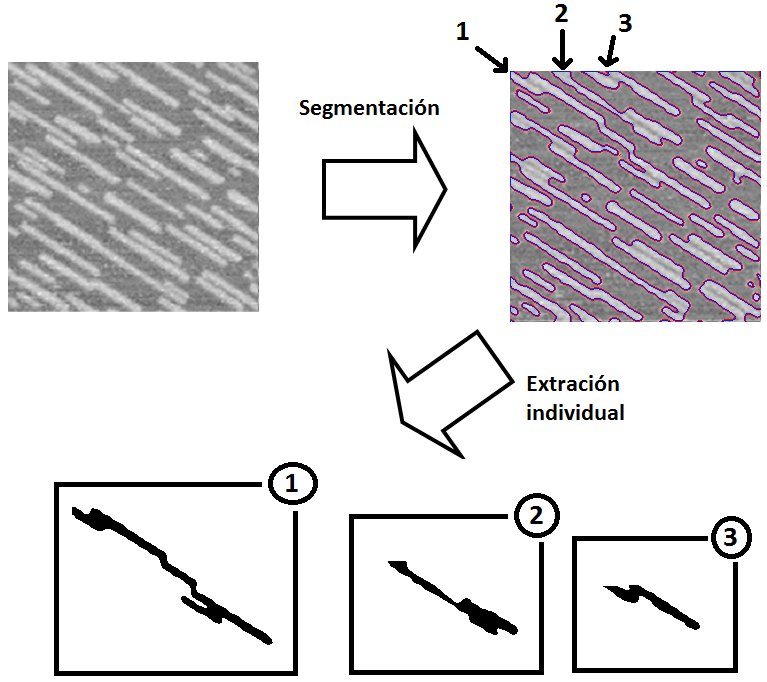
\includegraphics[width=1.1\textwidth]{./imagenes/extraccionIslaBuena}
	\caption{Proceso de extracci\'{o}n de las islas de la figura \ref{buena1} }	
	\label{extraccionIslaBuena}
\end{figure}



\section{Densidad}

Al cliente le interesa saber la densidad de las islas interiores y exteriores por separado, y realizar la media de los dos valores. Esta tarea se podr\'{a} hacer una vez realizada la extracci\'{o}n de las islas, es decir, la anterior tarea. El c\'{a}lculo de la densidad de todas las islas de la imagen ser\'{i}a sencilla, ya que una vez que se hayan extra\'{i}do \'{u}nicamente habr\'{a} que realizar la divisi\'{o}n: n\'{u}mero de islas entre el \'{a}rea total de la imagen.

 En cuanto a la primera cuesti\'{o}n, se deber\'{i}an de identificar las islas que est\'{a}n <<tocando>> los bordes o incluso que est\'{e}n incompletas. La soluci\'{o}n es realizar un conteo de las islas que no est\'{a}n en el borde a la par que se extraen, observando si alguna coordenada perteneciente al borde de las islas est\'{a} tocando el borde de la imagen. Una vez que tengamos el conteo se realizar\'{a} la misma divisi\'{o}n pero esta vez entre el n\'{u}mero de islas que no tocan la imagen y el \'{a}rea del marco en la que est\'{a}n circunscritas las islas. Para finalizar se realiza la media entre las dos densidades obtenidas.

\section{Power Spectral Density (PSD)}

\textit{Power Spectral Density}, o la densidad espectral de potencia en castellano, es una medida de la intensidad de la potencia de una se\~{n}al en el dominio de la frecuencia, informando de la distribuci\'{o}n de sus distintas componentes frecuenciales en el espectro. El resultado del PSD es una especie de <<mapa>> sobre las intensidades que tiene la imagen. Si entrar en m\'{a}s detalles sobre el PSD, el cliente tiene una herramienta en Java que realiza el PSD, por lo que se tendr\'{a}n que adaptar las im\'{a}genes de las islas extra\'{i}das (todas del mismo tama\~{n}o y cuadradas) de manera que se pueda realizar sin problemas.

Se realizar\'{a} el PSD de cada isla extra\'{i}da y se calcular\'{a} su promedio. Tambi\'{e}n se realizar\'{a} la misma acci\'{o}n pero esta vez de la imagen entera sin las islas de los bordes, ya que el tener islas <<cortadas>> a\~{n}adir\'{i}an ruido al c\'{a}lculo del PSD. Por lo tanto, para esto \'{u}ltimo se deber\'{a} crear una imagen nueva a partir de las islas que no est\'{e}n tocando los bordes.
